\documentclass[conference]{IEEEtran}
\IEEEoverridecommandlockouts

\usepackage{cite}
\usepackage{amsmath,amssymb,amsfonts}
\usepackage{graphicx}
\usepackage{textcomp}
\usepackage{xcolor}
\usepackage{booktabs}
\usepackage{array}
\usepackage{tikz}
\usetikzlibrary{arrows.meta}

\def\BibTeX{{\rm B\kern-.05em{\sc i\kern-.025em b}\kern-.08em
    T\kern-.1667em\lower.7ex\hbox{E}\kern-.125em X}}

\newcommand{\phihat}{\hat{\phi}}
\newcommand{\Ex}{\mathbb{E}}

\begin{document}

\title{How Cheaply Can Shapley Attributions Be Estimated? Five Model-Agnostic Estimators Measured Against Exact Values}

\author{
\IEEEauthorblockN{Ayushman Bhatt}
\IEEEauthorblockA{\textit{Dept.\ of Artificial Intelligence} \\
\textit{Sardar Vallabhbhai National Institute of Technology}\\
Surat, India \\
ayushman.bhatt.nitsurat@gmail.com}
\and
\IEEEauthorblockN{Arpit Mishra}
\IEEEauthorblockA{\textit{Dept.\ of Artificial Intelligence} \\
\textit{Sardar Vallabhbhai National Institute of Technology}\\
Surat, India \\
tech.toarpit@gmail.com}
}

\maketitle

\begin{abstract}
Shapley values split a model's prediction among its input features. The definition requires evaluating the model on every subset of the features, and the number of subsets doubles with each added feature, so the values are usually estimated. We implemented five model-agnostic estimators from scratch (permutation sampling, its antithetic variant, KernelSHAP, paired KernelSHAP and a multilinear-extension sampler) and compared them with exact values on a twelve-feature gradient boosting classifier, where all 4096 coalitions can still be enumerated. Paired KernelSHAP was the most accurate at every budget we tried. With 2048 coalition evaluations, half of what exact computation needs, its relative error was 0.76\%, about 63\% lower than that of permutation sampling, and it matched permutation sampling's final accuracy with roughly one sixth of the evaluations. The same ordering held at sixteen features. A multilinear estimator with a four-point grid was competitive at small budgets but kept a bias that additional samples did not remove; a finer grid removed most of it once the budget was large enough. We also checked three assumptions that explanation studies often leave untested. The selected features were strongly collinear (mean absolute correlation 0.78), the choice of background sample moved the exact values roughly twenty times more than the best estimator's error, and replicate-based confidence intervals covered the exact values close to their nominal rate. For the unpaired estimators the ranking settled before the values did, so a correct top-three list can still come with errors above five percent.
\end{abstract}

\begin{IEEEkeywords}
explainable AI, Shapley value, feature attribution, KernelSHAP, Monte Carlo estimation, variance reduction
\end{IEEEkeywords}

\section{Introduction}
If a model flags a tissue sample as malignant, a clinician may want to know which inputs led to that result. Feature attribution methods answer this by assigning each input a share of the prediction. The Shapley value \cite{shapley1953} is the only allocation that satisfies a set of fairness axioms, and since it was applied to machine learning \cite{strumbelj2014,lundberg2017} it has been widely used.

The definition is expensive to compute. The value of one feature is a weighted average over every subset of the remaining features, so a model with $d$ inputs has to be queried on $2^d$ coalitions for every single explanation. Exact computation is infeasible beyond a few dozen features, and often well before that. Most practical uses of Shapley values therefore rely on approximations, and a recent survey counted two dozen distinct estimation algorithms \cite{chen2023algorithms}, and newer estimators with accuracy guarantees have been proposed \cite{musco2025,witter2025}.

Theory can compare these methods, but some practical questions need measurements. How many model evaluations does each estimator need to reach a given accuracy? Does an accurate value mean a correct ranking of features, which is what most readers of an attribution plot look at? And how much does the error against exact values matter, given that the value function is itself a modelling choice? Answering these requires ground truth, so we work at sizes where brute force is still possible.

This paper reports such a study. Our contributions are:
\begin{itemize}
\item a from-scratch implementation of five model-agnostic estimators evaluated under a common budget of coalition evaluations, with exact values as reference at $d=12$ and $d=16$;
\item a measurement of how exact computation scales, and of the budget at which each sampling estimator catches up with the others;
\item a bias--variance decomposition that separates the sampling noise of the multilinear estimator from its quadrature bias;
\item checks on three assumptions that attribution studies often take for granted: feature independence, the effect of the background sample, and the reliability of simple uncertainty estimates.
\end{itemize}
Code, raw runs and all tables are included with the submission so that every number below can be regenerated.

\section{System Architecture}
\label{sec:arch}
Fig.~\ref{fig:arch} summarises the whole study as a four-stage pipeline. \emph{Stage~1} builds the model to be explained: the diagnostic data are split, the $d$ most informative features are chosen on the training part only, and a gradient boosting classifier is fitted on them. \emph{Stage~2} turns the model into a cooperative game. A fixed background sample defines the interventional value function \eqref{eq:vf}, which is tabulated once for all $2^d$ coalitions of every explained instance; the exact Shapley values computed from that table are the ground truth. \emph{Stage~3} runs the five estimators under the common budget $m$ of coalition lookups, with independent random seeds. \emph{Stage~4} compares every estimate with the exact values using three metrics and feeds two groups of experiments: the benchmark itself (accuracy, scaling, the multilinear study), and the audits of the assumptions behind it (feature dependence, background sensitivity, interval coverage, a convergence check). Because estimators and exact values read the same table, any difference between them is estimation error and not a result of implementation differences.

\begin{figure*}[t]
\centering
\resizebox{\textwidth}{!}{%
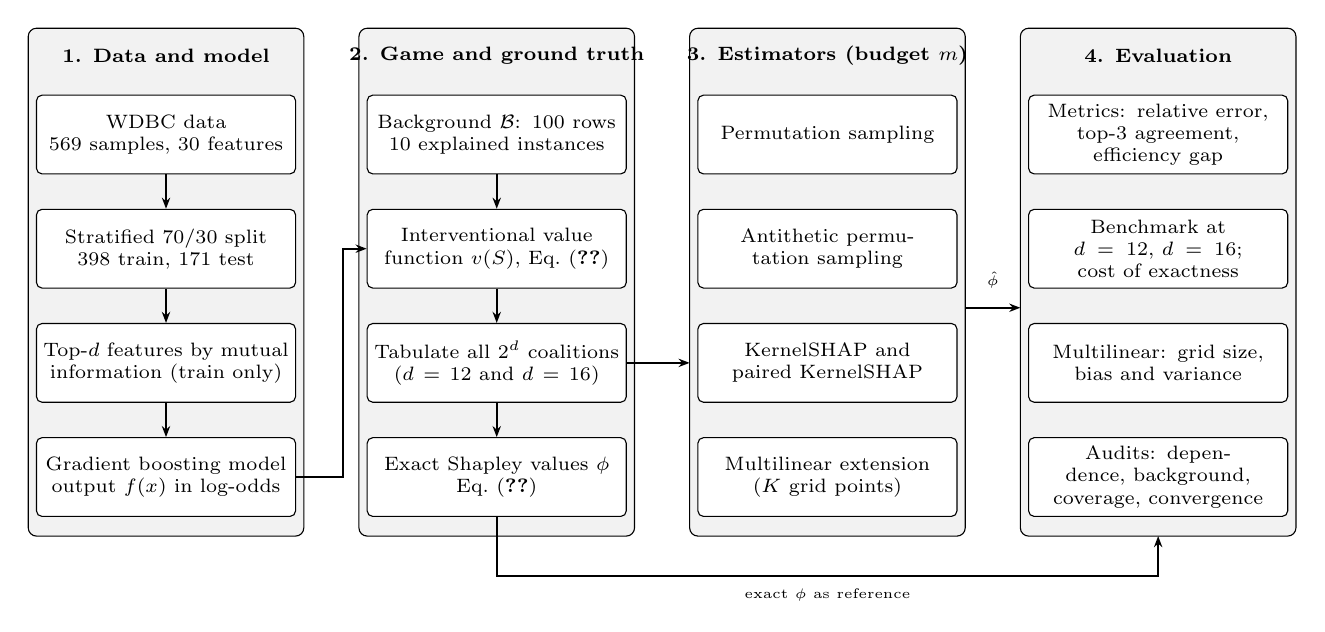
\begin{tikzpicture}[
  font=\scriptsize,
  box/.style={draw, rounded corners=2pt, align=center, minimum height=1.0cm, text width=3.15cm, inner sep=2pt, fill=white},
  panel/.style={draw, rounded corners=3pt, fill=gray!10},
  ttl/.style={font=\scriptsize\bfseries},
  arr/.style={-{Stealth[length=4pt]}, thick},
  lab/.style={font=\tiny, align=center}
]
% panels
\foreach \x in {0,4.2,8.4,12.6}{
  \draw[panel] (\x-1.75,-5.1) rectangle (\x+1.75,1.35);
}
\node[ttl] at (0,1.0) {1. Data and model};
\node[ttl] at (4.2,1.0) {2. Game and ground truth};
\node[ttl] at (8.4,1.0) {3. Estimators (budget $m$)};
\node[ttl] at (12.6,1.0) {4. Evaluation};
% stage 1
\node[box] (a1) at (0,0)     {WDBC data\\569 samples, 30 features};
\node[box] (a2) at (0,-1.45) {Stratified 70/30 split\\398 train, 171 test};
\node[box] (a3) at (0,-2.9)  {Top-$d$ features by mutual\\information (train only)};
\node[box] (a4) at (0,-4.35) {Gradient boosting model\\output $f(x)$ in log-odds};
\draw[arr] (a1) -- (a2); \draw[arr] (a2) -- (a3); \draw[arr] (a3) -- (a4);
% stage 2
\node[box] (b1) at (4.2,0)     {Background $\mathcal{B}$: 100 rows\\10 explained instances};
\node[box] (b2) at (4.2,-1.45) {Interventional value\\function $v(S)$, Eq.~\eqref{eq:vf}};
\node[box] (b3) at (4.2,-2.9)  {Tabulate all $2^d$ coalitions\\($d=12$ and $d=16$)};
\node[box] (b4) at (4.2,-4.35) {Exact Shapley values $\phi$\\Eq.~\eqref{eq:shapley}};
\draw[arr] (b1) -- (b2); \draw[arr] (b2) -- (b3); \draw[arr] (b3) -- (b4);
\draw[arr] (a4.east) -- ++(0.6,0) |- (b2.west);
% stage 3
\node[box] (c1) at (8.4,0)     {Permutation sampling};
\node[box] (c2) at (8.4,-1.45) {Antithetic permutation sampling};
\node[box] (c3) at (8.4,-2.9)  {KernelSHAP and\\paired KernelSHAP};
\node[box] (c4) at (8.4,-4.35) {Multilinear extension\\($K$ grid points)};
\draw[arr] (b3.east) -- (6.65,-2.9);
% stage 4
\node[box] (d1) at (12.6,0)     {Metrics: relative error,\\top-3 agreement, efficiency gap};
\node[box] (d2) at (12.6,-1.45) {Benchmark at $d=12$, $d=16$;\\cost of exactness};
\node[box] (d3) at (12.6,-2.9)  {Multilinear: grid size,\\bias and variance};
\node[box] (d4) at (12.6,-4.35) {Audits: dependence, background,\\coverage, convergence};
\draw[arr] (10.15,-2.2) -- (10.85,-2.2);
\node[lab] at (10.5,-1.85) {$\hat\phi$};
% exact values as reference
\draw[arr] (b4.south) -- ++(0,-0.75) -| (12.6,-5.1);
\node[lab, fill=white, inner sep=1pt] at (8.4,-5.85) {exact $\phi$ as reference};
\end{tikzpicture}}
\caption{System architecture of the study. The model of Stage~1 is turned into a tabulated game in Stage~2; all five estimators in Stage~3 read from the same table (20 seeds per instance), and Stage~4 compares their output with the exact values and runs the follow-up experiments of Section~\ref{sec:results}.}
\label{fig:arch}
\end{figure*}

\section{Background}

\subsection{The Shapley value}
Let $N=\{1,\dots,d\}$ be the set of players and let $v:2^N\to\mathbb{R}$ assign a payoff to every coalition. The Shapley value of player $i$ is
\begin{equation}
\phi_i = \sum_{S\subseteq N\setminus\{i\}} \frac{|S|!\,(d-|S|-1)!}{d!}\,\bigl[v(S\cup\{i\})-v(S)\bigr].
\label{eq:shapley}
\end{equation}
The weight is the probability that player $i$ arrives right after the members of $S$ when the players enter in a uniformly random order. The values satisfy efficiency, $\sum_i\phi_i=v(N)-v(\emptyset)$, together with symmetry, a null-player property and linearity, and they are the only values that do \cite{shapley1953}.

Equation~\eqref{eq:shapley} can be rewritten in two ways that matter for estimation. As an average over orderings $\pi$ of the players,
\begin{equation}
\phi_i = \frac{1}{d!}\sum_{\pi}\bigl[v(P_i^\pi\cup\{i\})-v(P_i^\pi)\bigr],
\label{eq:perm}
\end{equation}
where $P_i^\pi$ holds the players that precede $i$ in $\pi$. And as the solution of a weighted least-squares problem \cite{lundberg2017},
\begin{equation}
\begin{split}
\phi=\arg\min_{\beta}\sum_{z\in\{0,1\}^d}&\pi(z)\Bigl[v(z)-v(\emptyset)-\sum_i\beta_i z_i\Bigr]^2\\
&\text{s.t.}\ \sum_i\beta_i=v(N)-v(\emptyset),
\end{split}
\label{eq:wls}
\end{equation}
with the Shapley kernel $\pi(z)=(d-1)/\bigl[\binom{d}{|z|}\,|z|\,(d-|z|)\bigr]$. A third form, Owen's multilinear extension \cite{owen1972}, writes $\phi_i$ as an integral over the probability $q$ with which each other player joins a coalition. Each form suggests its own family of estimators.

\subsection{From a prediction to a game}
A model $f$ is defined on complete inputs, so $v(S)$ must say what it means to know only the features in $S$. We use the interventional choice \cite{janzing2020,covert2021removal}: features outside $S$ are filled in with values from a background sample $\mathcal{B}$,
\begin{equation}
v(S)=\frac{1}{|\mathcal{B}|}\sum_{b\in\mathcal{B}} f\bigl(x_S,\,b_{N\setminus S}\bigr).
\label{eq:vf}
\end{equation}
Each coalition value therefore costs $|\mathcal{B}|$ forward passes. The alternative, conditioning on the observed features, respects the data distribution but needs a model of the joint distribution \cite{aas2021,frye2021}. We return to this choice in Section~\ref{sec:valuefn}, because it affected the results more than we expected.

\subsection{Approximation families}
Sampling orderings and averaging marginal contributions is the oldest approach \cite{strumbelj2014}. Hoeffding-type bounds give an error that falls as $1/\sqrt{m}$ in the number of samples \cite{maleki2013}, so the practical gains come from reducing the constant, for instance with antithetic or stratified designs \cite{mitchell2022} or by avoiding marginal contributions altogether \cite{kolpaczki2024,fumagalli2023}. KernelSHAP samples coalitions from the Shapley kernel and solves \eqref{eq:wls} on the sample; the paired variant that uses each coalition together with its complement reduces variance \cite{covert2021kernel}, and recent work improves the weighting of coalitions \cite{olsen2024} or replaces the sampling distribution by leverage scores, which gives non-asymptotic guarantees \cite{musco2025}. Regression-adjusted Monte Carlo estimators combine both ideas \cite{witter2025}, and the same machinery extends to Shapley interactions \cite{fumagalli2023,fumagalli2024}, and an open-source library implements them \cite{muschalik2024}. Multilinear sampling integrates over $q$ by quadrature \cite{okhrati2021}. If model structure may be used, TreeSHAP computes exact values for tree ensembles in polynomial time \cite{lundberg2020trees}, and amortised explainers trade accuracy for a single forward pass per explanation \cite{jethani2022}. Computing SHAP values exactly is intractable in general, even for simple model classes, once feature distributions are involved \cite{vandenbroeck2021}. This paper studies only the model-agnostic sampling estimators, since those are the ones that apply when the model is a black box.

\section{Estimators and Budget Accounting}
\label{sec:estimators}
The budget $m$ is the number of coalition values $v(S)$ an estimator may look up. The values $v(\emptyset)$ and $v(N)$ are free, since they equal the mean prediction on the background and the prediction itself. All five estimators below work from this common currency, so that none gains from implementation details.

\textbf{Permutation sampling.} Draw $\lfloor m/(d+1)\rfloor$ random orderings and average the terms of \eqref{eq:perm} over them. Walking along an ordering and adding one feature at a time costs $d+1$ lookups and yields one marginal contribution per feature; the estimate is the average over orderings.

\textbf{Antithetic permutation sampling.} Each drawn ordering is used together with its reverse, so $\lfloor m/(2(d+1))\rfloor$ pairs are used. A feature that enters early in one ordering enters late in the other, which makes the two contributions negatively correlated.

\textbf{KernelSHAP.} Draw $m$ coalitions. The size $s\in\{1,\dots,d-1\}$ is chosen with probability proportional to $(d-1)/(s(d-s))$, and the members are a uniformly random subset of that size. The constrained problem \eqref{eq:wls} is solved by least squares after eliminating one coefficient through the efficiency constraint, so $\sum_i\hat\phi_i=v(N)-v(\emptyset)$ holds exactly for any sample.

\textbf{Paired KernelSHAP.} Draw $m/2$ coalitions in the same way and add the complement $N\setminus S$ of each, for $m$ lookups in total, then solve the same constrained problem.

\textbf{Multilinear extension.} Place $K$ equally spaced grid points on $q\in[0,1]$. At a grid point, a sample draws each feature independently with probability $q$ to form a coalition $z$ and evaluates $z$ together with its $d$ single-feature flips ($d+1$ lookups); the marginal contribution of feature $i$ is the difference between the two coalitions that differ only in $i$. The endpoints $q=0$ and $q=1$ are deterministic and need one sample each. The remaining $\lfloor m/(d+1)\rfloor-2$ samples are spread over the $K-2$ interior points, and the integral is evaluated with the trapezoid rule. If the budget cannot give every interior point a sample, the estimator returns nothing. We use $K=4$ unless stated otherwise.

\section{Experimental Setup}
\label{sec:setup}

\textbf{Data and model.} We used the Wisconsin Diagnostic Breast Cancer data \cite{street1993} as distributed with scikit-learn: 569 samples and 30 features. A stratified 70/30 split (398 training and 171 test samples, \texttt{random\_state=0}) was made first. The $d$ features with the highest mutual information with the label were then selected using the training part only. A histogram gradient boosting classifier (200 iterations, maximum depth 4) was fitted on those features. It classified 160 of the 171 test samples correctly (93.57\%). We explain the log-odds output of the model, which is unbounded and tends to behave more additively than the probability.

\textbf{Ground truth.} The background sample $\mathcal{B}$ consists of 100 training points drawn once without replacement. For each explained instance we evaluate \eqref{eq:vf} on all $2^d$ coalitions in chunks, store the values in a table, and compute \eqref{eq:shapley} exactly. Every estimator then reads from this table, which makes a lookup cost the same for all of them. The exact values satisfy efficiency to within $2\times10^{-15}$. As further checks, all five estimators recover the exact values of an additive toy game to machine precision, and exact Shapley values of a three-player non-additive game match a hand calculation.

\textbf{Protocol.} The main benchmark uses $d=12$ (4096 coalitions), 10 test instances chosen once at random, 20 random seeds per instance (seed $=1000i+s$ for instance $i$ and repetition $s$), and budgets $m\in\{64,128,256,512,1024,2048\}$. A second benchmark at $d=16$ (65\,536 coalitions) uses 5 instances, 10 seeds and budgets up to 8192. Results are first averaged over seeds within an instance, and we then report the mean and standard error across instances; every $\pm$ below is such a standard error over $n=10$ instances ($n=5$ at $d=16$).

\textbf{Metrics.} With exact values $\phi$ and an estimate $\hat\phi$ we report the relative error $\lVert\hat\phi-\phi\rVert_2/\lVert\phi\rVert_2$; the top-3 agreement, defined as the fraction of the three features with the largest exact $|\phi_i|$ that also appear among the three largest $|\hat\phi_i|$; and the efficiency gap $\bigl|\sum_i\hat\phi_i-(v(N)-v(\emptyset))\bigr|$.

\textbf{Environment.} All runs used Python 3.12.7, NumPy 1.26.4, SciPy 1.16.2 and scikit-learn 1.7.2 on a 16-thread AMD64 machine under Windows. The main benchmark and its follow-up phases take about four minutes in total; the additional studies in Sections~\ref{sec:valuefn}--\ref{sec:mlbias} take about twelve more.

\section{Results}
\label{sec:results}

\subsection{Accuracy at twelve features}
\begin{table*}[t]
\caption{Relative error against exact Shapley values, $d=12$ (mean $\pm$ s.e.\ over 10 instances; lower is better). The last column is the efficiency gap at $m=2048$ in log-odds units. Exact computation needs 4096 lookups.}
\label{tab:main}
\centering
\small
\resizebox{\textwidth}{!}{%
\begin{tabular}{lccccccc}
\toprule
Estimator & $m=64$ & $m=128$ & $m=256$ & $m=512$ & $m=1024$ & $m=2048$ & Eff.\ gap \\
\midrule
Permutation & $0.130\pm0.009$ & $0.086\pm0.006$ & $0.060\pm0.005$ & $0.040\pm0.003$ & $0.028\pm0.002$ & $0.020\pm0.002$ & $<10^{-14}$ \\
Antithetic perm.\ & $0.067\pm0.006$ & $0.046\pm0.005$ & $0.030\pm0.003$ & $0.021\pm0.002$ & $0.015\pm0.001$ & $0.010\pm0.001$ & $<10^{-14}$ \\
KernelSHAP & $0.125\pm0.009$ & $0.085\pm0.008$ & $0.057\pm0.005$ & $0.041\pm0.003$ & $0.029\pm0.002$ & $0.020\pm0.002$ & $<10^{-14}$ \\
Paired KernelSHAP & $\mathbf{0.055\pm0.005}$ & $\mathbf{0.033\pm0.003}$ & $\mathbf{0.023\pm0.002}$ & $\mathbf{0.016\pm0.002}$ & $\mathbf{0.011\pm0.001}$ & $\mathbf{0.008\pm0.001}$ & $<10^{-14}$ \\
Multilinear ($K=4$) & $0.112\pm0.008$ & $0.060\pm0.004$ & $0.037\pm0.003$ & $0.027\pm0.002$ & $0.020\pm0.001$ & $0.015\pm0.001$ & $0.110\pm0.010$ \\
\bottomrule
\end{tabular}}
\end{table*}

\begin{figure*}[t]
\centering
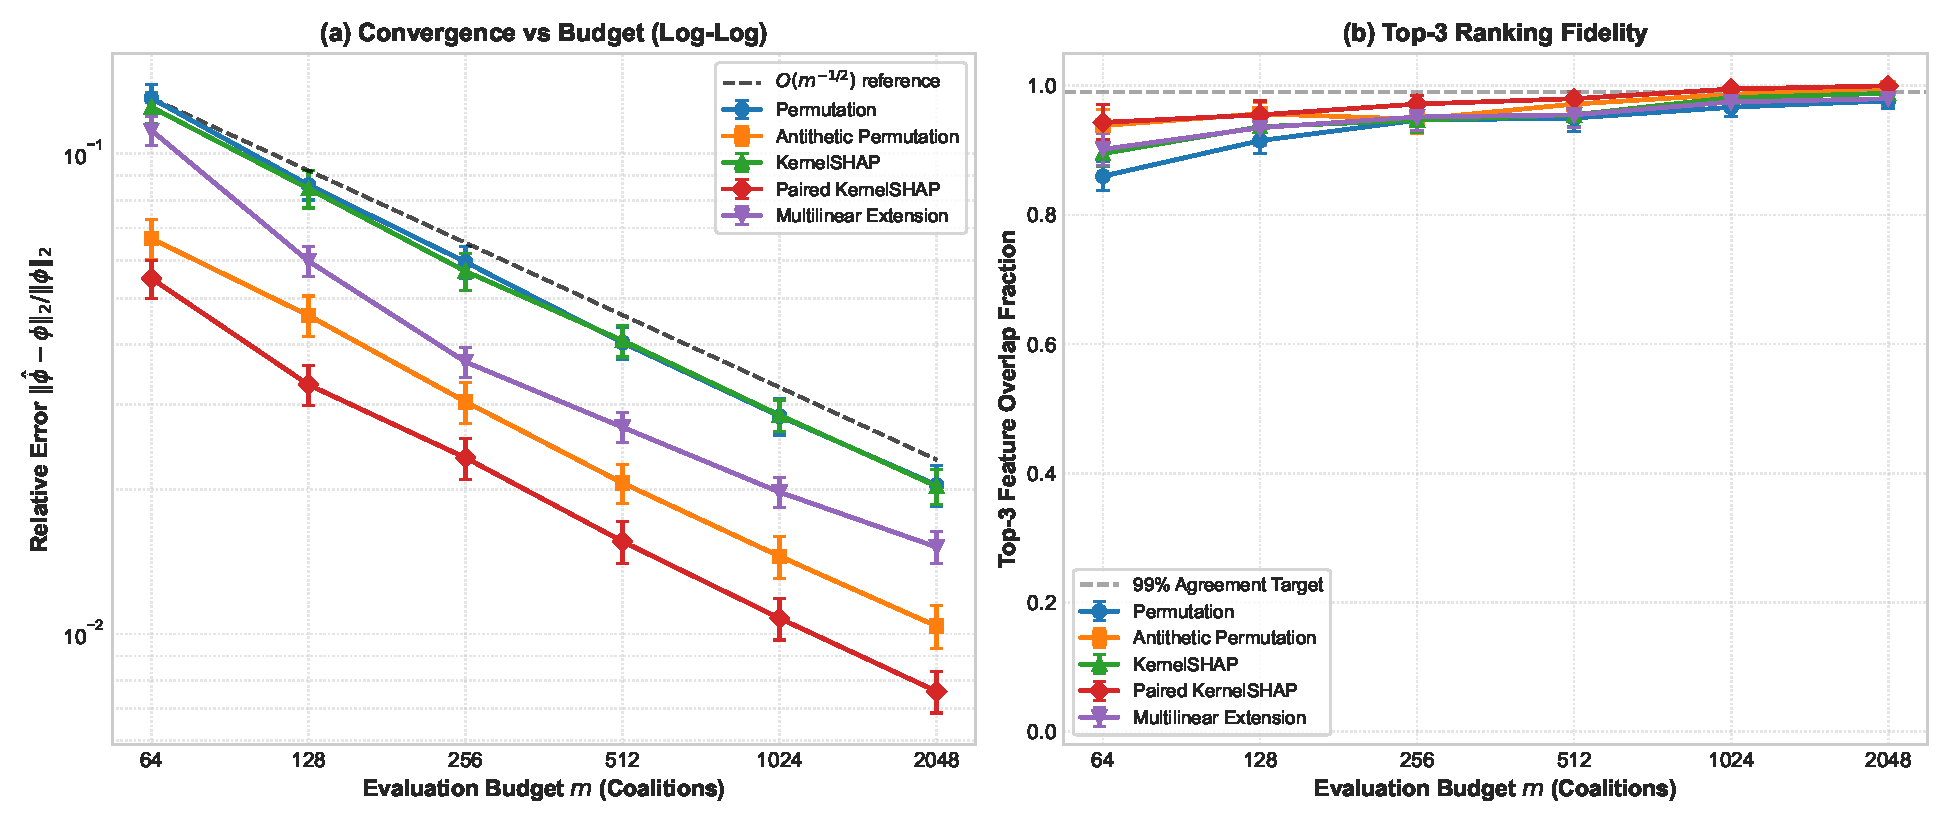
\includegraphics[width=\textwidth]{figures/figure1_main_benchmark.pdf}
\caption{Main benchmark at $d=12$. (a) Relative error against the exact Shapley values on log--log axes, with an $O(m^{-1/2})$ reference line anchored at the smallest budget. (b) Top-3 agreement; the dashed line marks 0.99. Error bars are standard errors over 10 instances.}
\label{fig:main}
\end{figure*}

Table~\ref{tab:main} and Fig.~\ref{fig:main} show the main comparison. Paired KernelSHAP has the lowest error at every budget. At $m=2048$ its relative error is $0.0076\pm0.0007$, against $0.0203\pm0.0017$ for KernelSHAP and $0.0204\pm0.0020$ for permutation sampling, reductions of 62.6\% and 62.8\%. Antithetic permutation sampling also gains from pairing, with a 49.2\% reduction over plain permutation sampling, but gains less than the paired regression. Plain KernelSHAP and plain permutation sampling are nearly indistinguishable at all budgets from 128 upward.

To express the gap as a saving, we interpolate each error curve in log--log space and ask how many evaluations an estimator needs to match the error permutation sampling reaches at $m=2048$. Paired KernelSHAP needs about 321, a factor of 6.4; antithetic permutation sampling needs 643 (3.2$\times$); the multilinear estimator needs 1123 (1.8$\times$); and plain KernelSHAP needs 2023, a saving of about 1\%.

All curves except the multilinear one run roughly parallel to the $m^{-1/2}$ line. The fitted log--log slopes are $-0.535$ (permutation), $-0.542$ (antithetic), $-0.523$ (KernelSHAP) and $-0.563$ (paired KernelSHAP), and the multilinear curve has slope $-0.562$ over this range. The slopes suggest that the rate is fixed and only the constant changes. A slope slightly steeper than $-0.5$ is within what 10 instances can resolve, and we do not read anything into it.

\begin{table}[t]
\caption{Top-3 agreement with the exact ranking, $d=12$ (mean over 10 instances; standard errors range from 0 to 0.03).}
\label{tab:top3}
\centering
\small
\resizebox{\columnwidth}{!}{%
\begin{tabular}{lcccc}
\toprule
Estimator & $m=64$ & $m=256$ & $m=512$ & $m=2048$ \\
\midrule
Permutation & 0.860 & 0.947 & 0.950 & 0.977 \\
Antithetic perm.\ & 0.938 & 0.948 & 0.972 & 0.997 \\
KernelSHAP & 0.895 & 0.947 & 0.955 & 0.988 \\
Paired KernelSHAP & \textbf{0.943} & \textbf{0.972} & \textbf{0.980} & \textbf{1.000} \\
Multilinear ($K=4$) & 0.902 & 0.952 & 0.955 & 0.980 \\
\bottomrule
\end{tabular}}
\end{table}

Rankings converge faster than values (Table~\ref{tab:top3}). Paired KernelSHAP recovers the exact top three features with agreement 0.98 at $m=512$, while its relative error there is still 1.6\%. It is the first estimator to pass 0.99, at $m=1024$ (0.995); antithetic permutation sampling gets there at 2048, and the other three have not reached 0.99 by 2048.

On efficiency, the permutation estimators satisfy the axiom to machine precision because each ordering telescopes to $v(N)-v(\emptyset)$, and both KernelSHAP variants satisfy it by construction. The multilinear estimator does not: its gap at $m=2048$ is $0.110\pm0.010$ log-odds units. Where that gap comes from is the subject of Section~\ref{sec:mlbias}.

\subsection{The cost of exactness}
\begin{figure}[t]
\centering
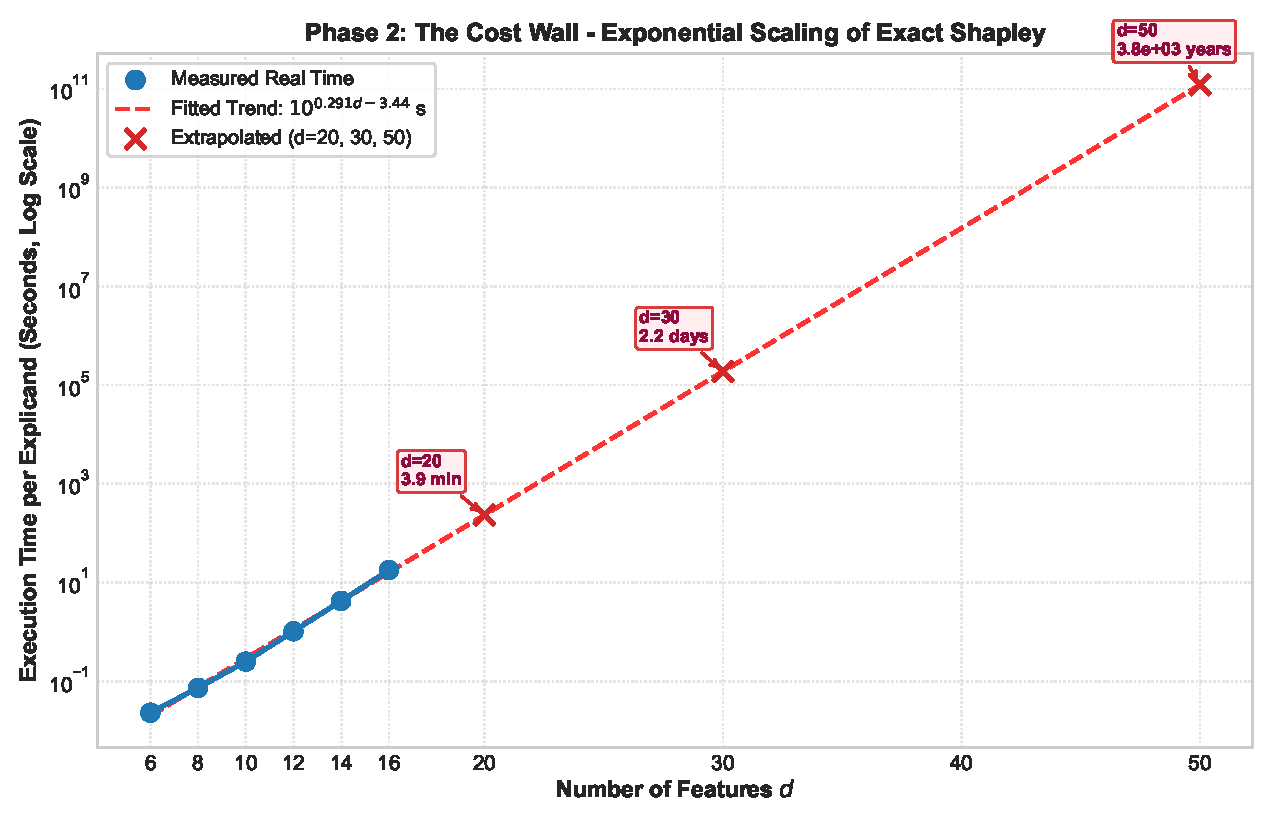
\includegraphics[width=\columnwidth]{figures/figure2_cost_wall.pdf}
\caption{Wall-clock time per instance of tabulating all $2^d$ coalitions against 100 background points and computing exact values. Measured for $d\le16$ (circles); crosses are extrapolations from the fitted line.}
\label{fig:cost}
\end{figure}

\begin{table}[t]
\caption{Cost of exact computation per explained instance ($|\mathcal{B}|=100$, one CPU process).}
\label{tab:cost}
\centering
\small
\resizebox{\columnwidth}{!}{%
\begin{tabular}{rrrr}
\toprule
$d$ & Coalitions & Forward passes & Time \\
\midrule
6 & 64 & $6.4\times10^{3}$ & 0.02 s \\
10 & 1024 & $1.0\times10^{5}$ & 0.25 s \\
12 & 4096 & $4.1\times10^{5}$ & 1.0 s \\
16 & 65\,536 & $6.6\times10^{6}$ & 17.8 s \\
20 & $1.0\times10^{6}$ & $1.0\times10^{8}$ & 3.9 min$^{\dagger}$ \\
30 & $1.1\times10^{9}$ & $1.1\times10^{11}$ & 2.2 days$^{\dagger}$ \\
50 & $1.1\times10^{15}$ & $1.1\times10^{17}$ & $3.8\times10^{3}$ years$^{\dagger}$ \\
\bottomrule
\multicolumn{4}{l}{\footnotesize $^{\dagger}$Extrapolated from the fit in Fig.~\ref{fig:cost}.}
\end{tabular}}
\end{table}

At $d=12$, exact computation needs 4096 coalition values, or 409\,600 forward passes with a background of 100, and took between 1.0 and 1.3 s per instance, depending on the run. Timings for $d=6,\dots,16$ lie on a straight line in a semi-log plot (Fig.~\ref{fig:cost}), with time growing by a factor of about 1.95 per added feature. Extrapolating that line gives minutes at $d=20$, days at $d=30$ and millennia at $d=50$ (Table~\ref{tab:cost}). These extrapolated figures describe our machine and this model, and they use a tabulation that does not exploit any structure of the model, but the exponential growth is what matters. Above roughly twenty features exact computation is not a realistic option for a black-box model.

\subsection{Scaling to sixteen features}
\begin{table}[t]
\caption{Relative error at $d=16$ (5 instances, 10 seeds; mean $\pm$ s.e.). Even $m=8192$ is one eighth of the 65\,536 coalitions.}
\label{tab:d16}
\centering
\small
\setlength{\tabcolsep}{3pt}
\resizebox{\columnwidth}{!}{%
\begin{tabular}{lccc}
\toprule
Estimator & $m=128$ & $m=1024$ & $m=8192$ \\
\midrule
Permutation & $0.0995\pm0.0130$ & $0.0314\pm0.0035$ & $0.0122\pm0.0014$ \\
Antithetic perm.\ & $0.0378\pm0.0050$ & $0.0108\pm0.0016$ & $0.0041\pm0.0007$ \\
KernelSHAP & $0.1055\pm0.0094$ & $0.0369\pm0.0023$ & $0.0126\pm0.0010$ \\
Paired KernelSHAP & $\mathbf{0.0330\pm0.0056}$ & $\mathbf{0.0102\pm0.0018}$ & $\mathbf{0.0035\pm0.0006}$ \\
Multilinear ($K=4$) & $0.0694\pm0.0072$ & $0.0213\pm0.0033$ & $0.0095\pm0.0013$ \\
\bottomrule
\end{tabular}}
\end{table}

\begin{figure*}[t]
\centering
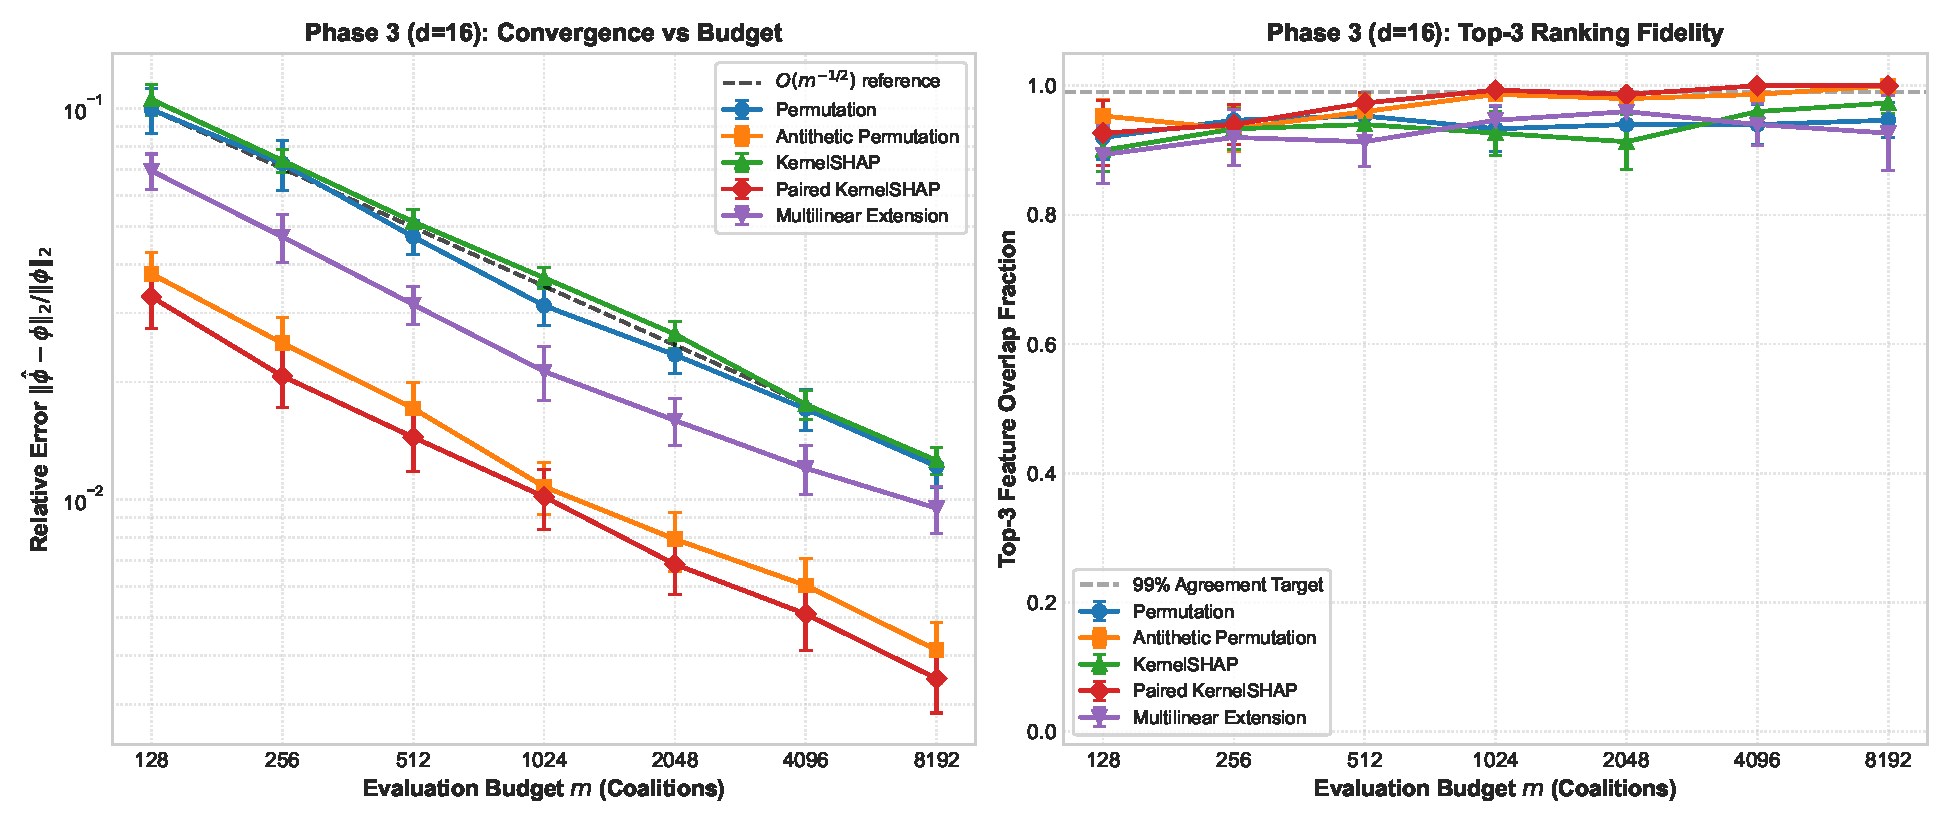
\includegraphics[width=\textwidth]{figures/figure3_scale_d16.pdf}
\caption{The benchmark repeated at $d=16$. Left: relative error against exact values. Right: top-3 agreement; with only five instances this panel is noisy and its curves should be read as a trend rather than a ranking.}
\label{fig:d16}
\end{figure*}

We repeated the comparison with the sixteen most informative features, where a budget of 128 is 0.2\% of the coalitions. The ordering is the same (Table~\ref{tab:d16}, Fig.~\ref{fig:d16}): paired KernelSHAP first, antithetic permutation sampling second, then the multilinear estimator, with permutation sampling and KernelSHAP last and close together. The advantage of the paired methods over their unpaired counterparts is larger here than at $d=12$. At $m=128$, antithetic permutation sampling has less than 40\% of the error of permutation sampling, and paired KernelSHAP has about a third of the error of KernelSHAP. The top-3 curves at $d=16$ rest on five instances and are noisy. Paired KernelSHAP is at 0.99 or above at $m=1024$, 4096 and 8192 (0.987 at $m=2048$), antithetic permutation sampling reaches 1.0 only at $m=8192$, and permutation sampling stays between 0.92 and 0.95 across the whole range. At $m=128$ antithetic permutation sampling is actually ahead of paired KernelSHAP on this metric (0.953 against 0.927).

\subsection{Multilinear grid size}
\label{sec:grid}
\begin{figure*}[t]
\centering
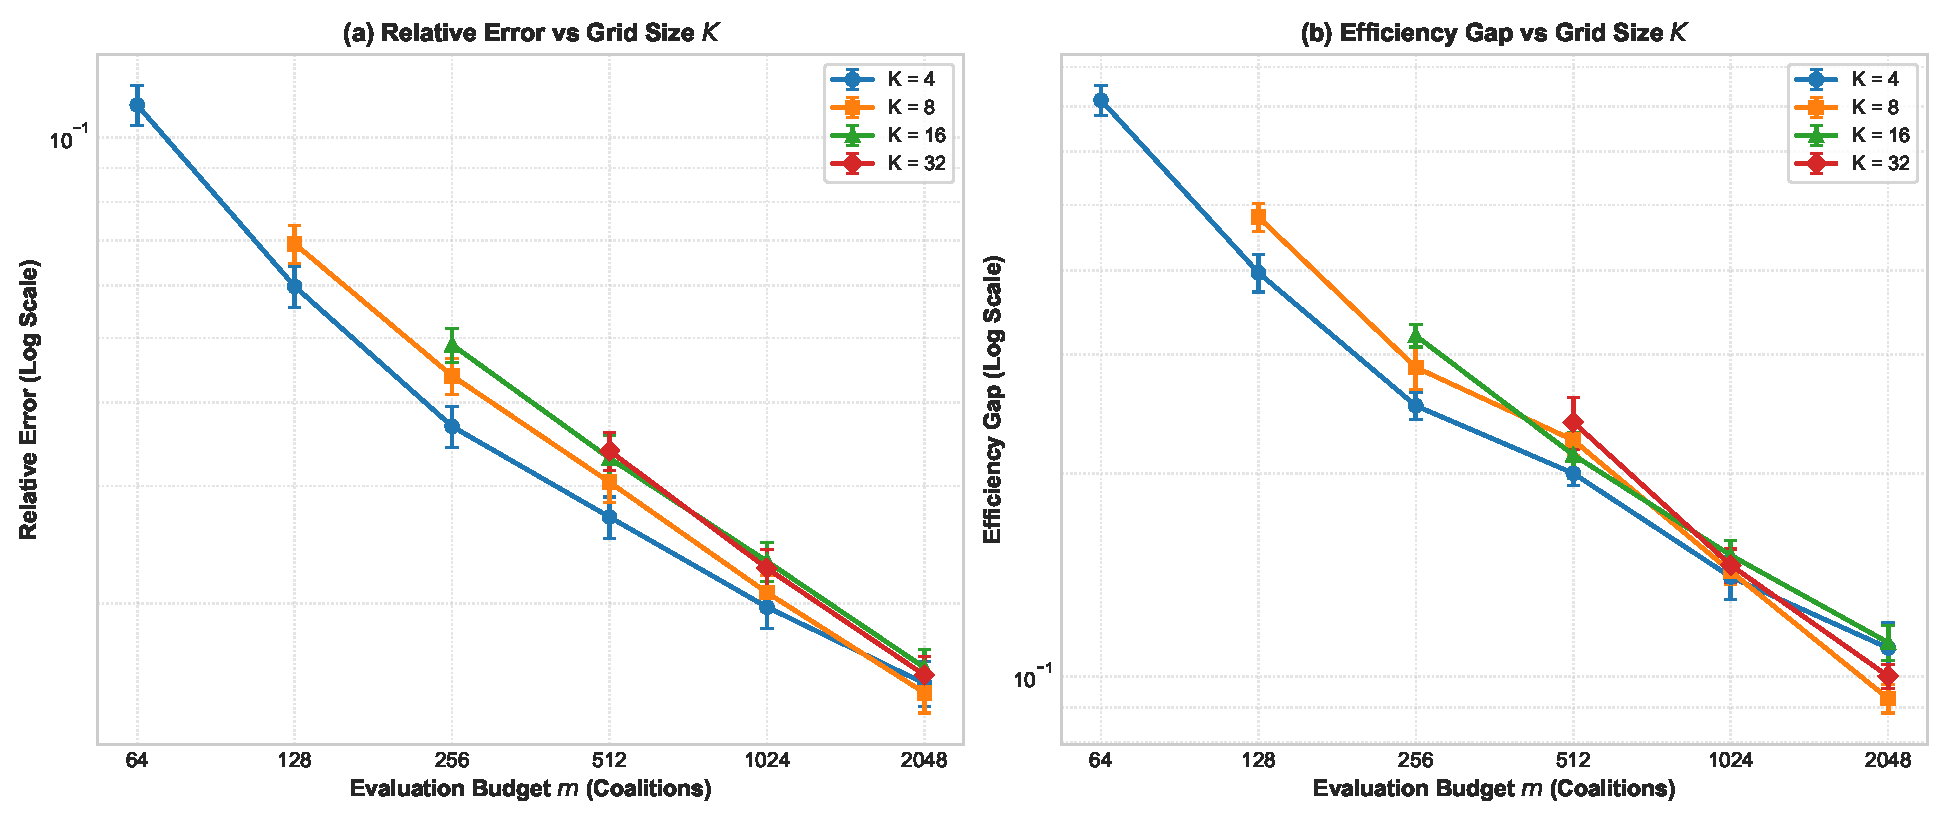
\includegraphics[width=\textwidth]{figures/figure4_multilinear_ablation.pdf}
\caption{Multilinear estimator at $d=12$ for grid sizes $K\in\{4,8,16,32\}$. A grid point is only plotted when the budget leaves at least one sample for every interior point. (a) Relative error. (b) Efficiency gap.}
\label{fig:grid}
\end{figure*}

A finer grid should reduce quadrature error, but the budget is fixed, so it also leaves fewer samples per grid point. Figure~\ref{fig:grid} shows that effect. For $K=16$ and $K=32$ the estimator cannot run at all until $m=256$ and $m=512$, respectively, and where both run, the coarse grid is better at small budgets: at $m=512$ the relative errors are 0.027 ($K=4$), 0.030 ($K=8$), 0.033 ($K=16$) and 0.034 ($K=32$). By $m=2048$ the curves have nearly converged (0.015--0.016) and the efficiency gap is 0.110 for $K=4$ and 0.100 for $K=32$. From this ablation alone one cannot tell whether the remaining gap is bias or noise, because both depend on the grid and on the number of samples. Section~\ref{sec:mlbias} separates them.

\subsection{Is the multilinear gap bias or noise?}
\label{sec:mlbias}
\begin{figure*}[t]
\centering
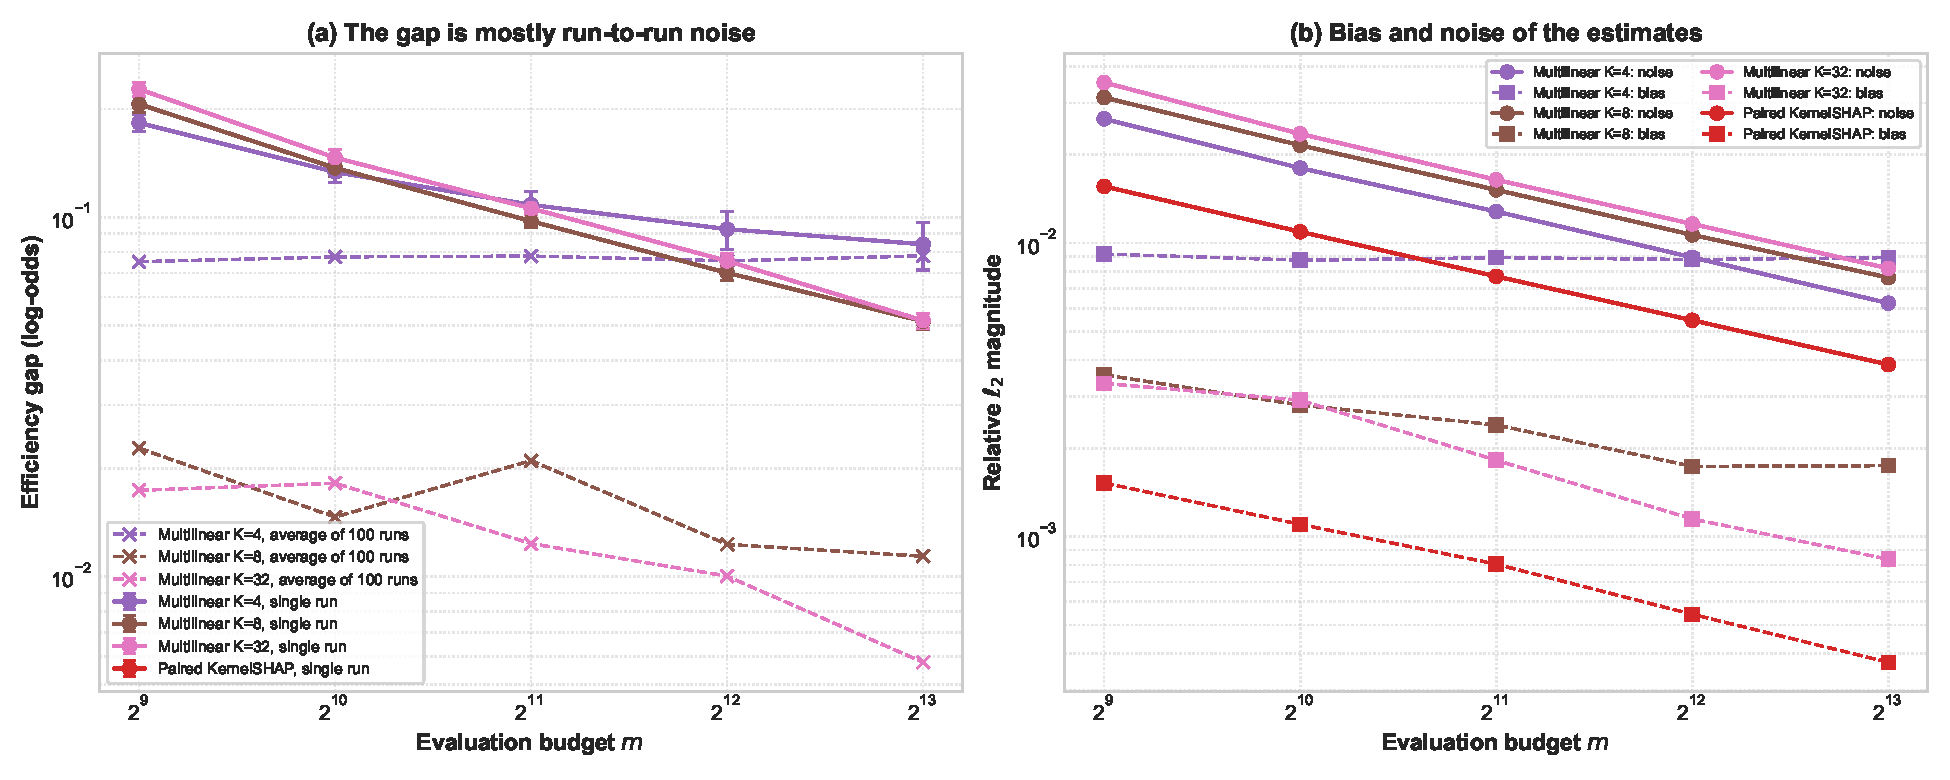
\includegraphics[width=\textwidth]{figures/figure9_multilinear_bias_variance.pdf}
\caption{Bias--variance decomposition of the multilinear estimator, 100 replicates per instance and budget ($d=12$). (a) Efficiency gap of a single run (solid) and of the average of 100 runs (dashed); the average isolates the bias. Paired KernelSHAP has gap exactly zero and is therefore not visible on the logarithmic axis. (b) Noise (solid) and bias (dashed) of the estimates in relative $\ell_2$ terms.}
\label{fig:mlbias}
\end{figure*}

\begin{table}[t]
\caption{Decomposition of the error of the multilinear estimator ($d=12$, 100 replicates $\times$ 10 instances). Bias and noise are relative $\ell_2$ magnitudes; the efficiency gap is in log-odds units.}
\label{tab:mlbias}
\centering
\small
\setlength{\tabcolsep}{3pt}
\resizebox{\columnwidth}{!}{%
\begin{tabular}{llcccc}
\toprule
 & $m$ & Run error & Bias & Eff.\ gap (run) & Eff.\ gap (mean) \\
\midrule
$K=4$ & 512 & 0.027 & 0.0092 & 0.183 & 0.075 \\
 & 8192 & 0.011 & 0.0089 & 0.084 & 0.078 \\
$K=8$ & 512 & 0.030 & 0.0036 & 0.206 & 0.023 \\
 & 8192 & 0.0075 & 0.0017 & 0.051 & 0.011 \\
$K=32$ & 512 & 0.034 & 0.0033 & 0.227 & 0.017 \\
 & 8192 & 0.0079 & 0.0008 & 0.052 & 0.006 \\
Paired KS & 512 & 0.015 & 0.0015 & 0 & 0 \\
 & 8192 & 0.0038 & 0.0004 & 0 & 0 \\
\bottomrule
\end{tabular}}
\end{table}

If an estimator is run many times on the same instance, the average of its outputs approximates its expected value, and the squared error of a single run splits into the squared distance of that average from the truth (bias) and the spread of runs around it (noise). We did this with 100 runs for each instance and budget, for $K=4,8,32$ and for paired KernelSHAP as a reference (Fig.~\ref{fig:mlbias} and Table~\ref{tab:mlbias}). A gap that remains in the \emph{average} of runs cannot be sampling noise.

For $K=4$ the answer is mixed. Bias is flat in the budget (0.0092 at $m=512$ and 0.0089 at $m=8192$; fitted slope $-0.01$), and the efficiency gap of the averaged estimate stays between 0.075 and 0.078 at every budget. This is a floor set by the quadrature error. The noise falls below it at about $m=4096$ (at $m=8192$ the bias is 0.0089 and the noise 0.0062), after which the estimator stops improving. The gap of a single run is larger than the floor, and it decreases with $m$ only because its noise part does. With four grid points the estimator is therefore bias-limited from roughly $m=4096$ on, and the floor does not depend on the sampling budget.

For $K=8$ and $K=32$ the picture changes. The bias is small (0.0017 and 0.0008 at $m=8192$, close to the 0.0008 that 100 replicates could resolve on their own), the efficiency gap of the average is at most 0.023, and the single-run gap falls at close to the Monte Carlo rate (slope $-0.50$ and $-0.52$). For these grids the efficiency gap seen in a single run is mostly noise. A finer grid also has the best final error: at $m=8192$ the relative error is 0.0075 for $K=8$, 0.0079 for $K=32$ and 0.0108 for $K=4$, against 0.0038 for paired KernelSHAP. The multilinear estimator therefore improves with a finer grid, but only once the budget is large enough to feed it, and it still does not satisfy efficiency for any finite sample, which both KernelSHAP variants do.

\subsection{A cheap convergence check}
\begin{figure*}[t]
\centering
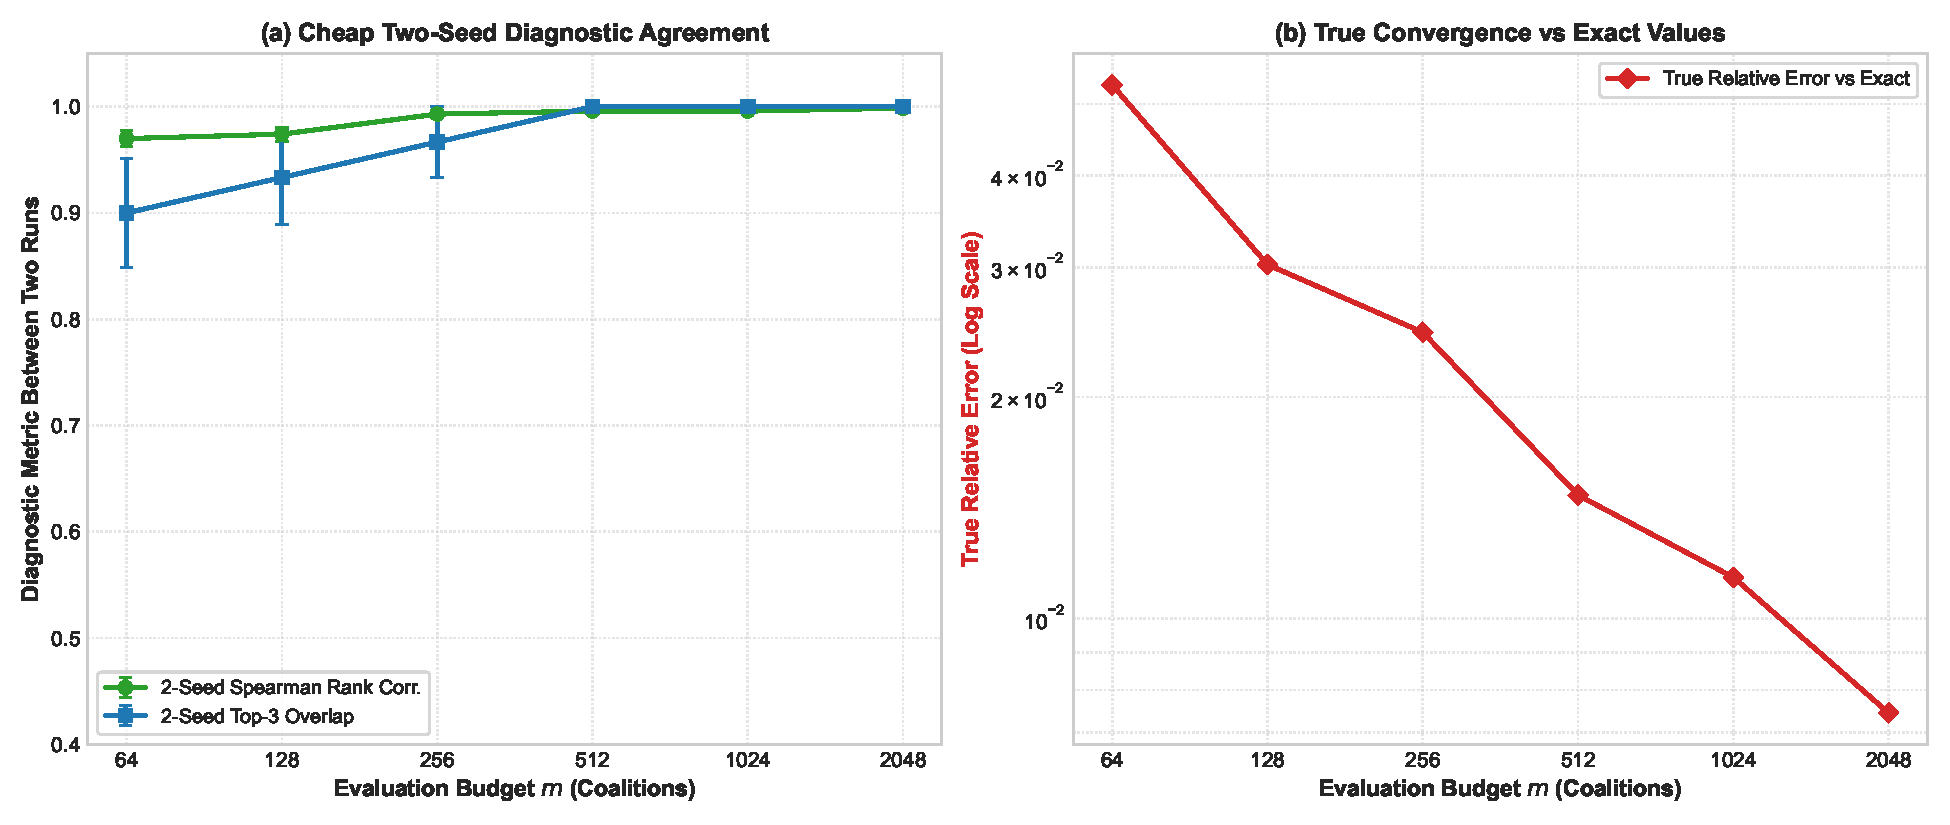
\includegraphics[width=\textwidth]{figures/figure5_convergence_check.pdf}
\caption{Two-run diagnostic for paired KernelSHAP. (a) Agreement between two independent runs on the same instance: top-3 overlap and Spearman correlation of absolute attributions. (b) The true relative error against exact values, which would be unknown in practice.}
\label{fig:conv}
\end{figure*}

In deployment the exact values are not available, so the error cannot be computed. A cheap proxy is to run the estimator twice with different seeds and compare. We tried this for paired KernelSHAP on the 10 instances, using one pair of seeds per instance and budget (Fig.~\ref{fig:conv}). At $m\ge512$ the two runs agreed on the same top three features for all 10 instances, their Spearman correlation was at least 0.995, and the true relative error was at most 1.5\%; the true top three were also recovered for all 10 instances. At $m=256$ the two-run agreement was already 0.967 and the Spearman correlation 0.993, but the true top-3 agreement was 0.95, so agreement between runs overstated reliability at that budget. Because this uses only one pair of seeds per instance, we treat it as a plausibility check, not a calibrated stopping rule.

\subsection{How dependent are the features?}
\label{sec:dep}
\begin{figure*}[t]
\centering
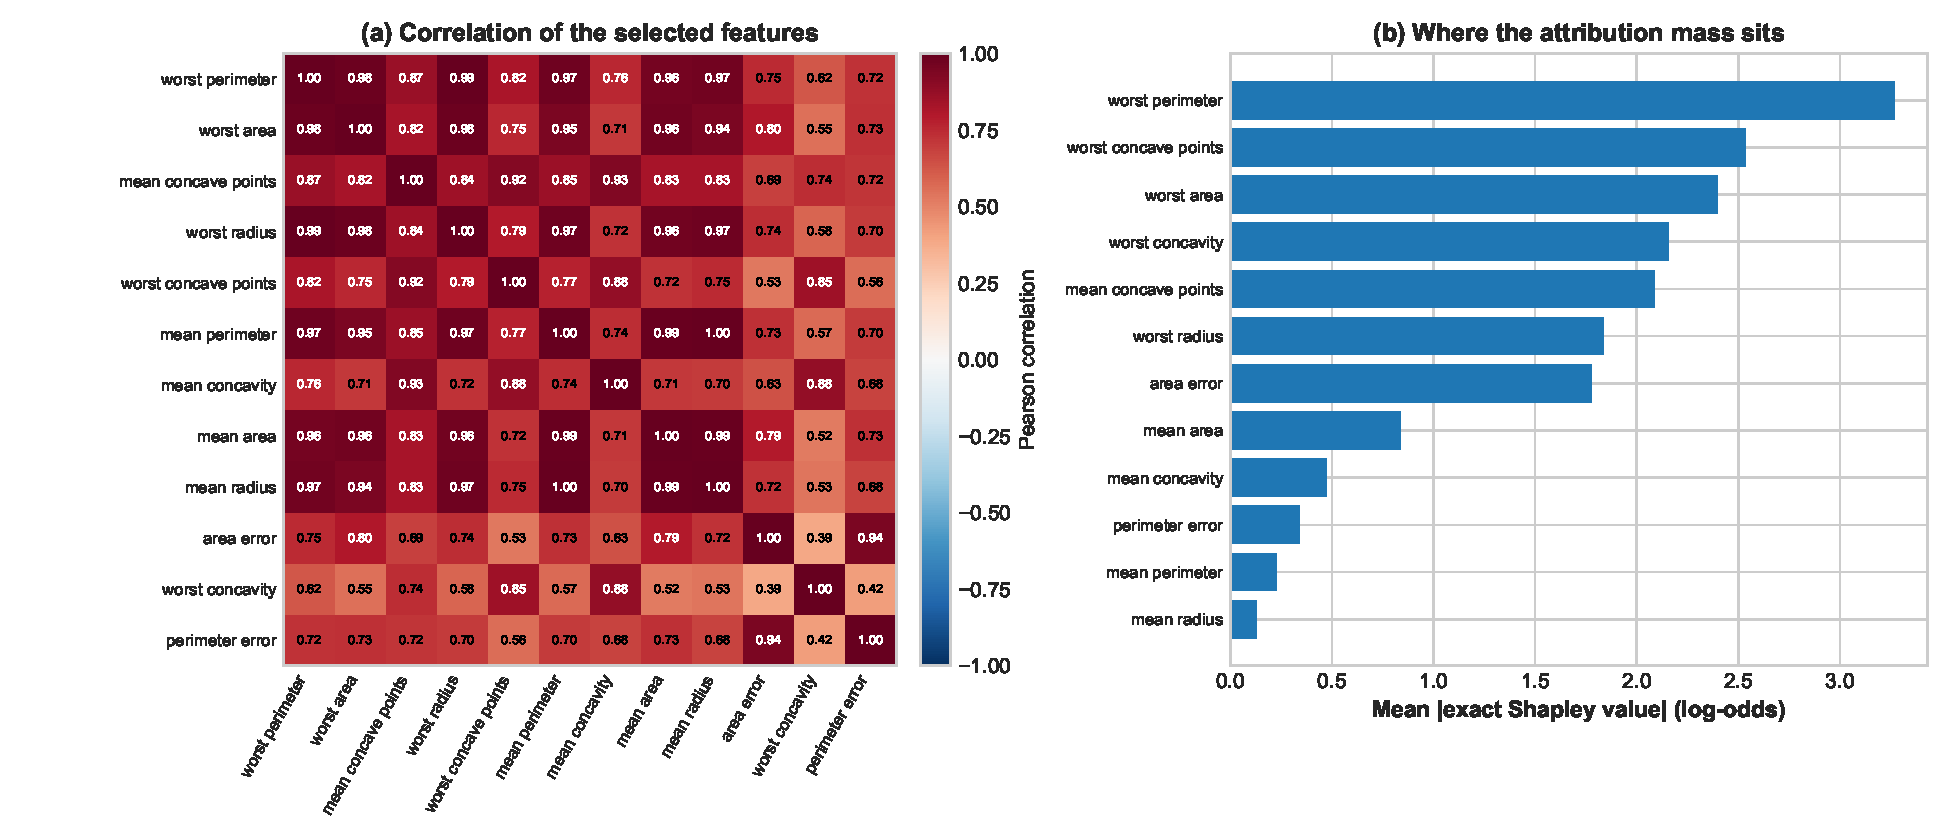
\includegraphics[width=\textwidth]{figures/figure6_feature_dependence.pdf}
\caption{(a) Pearson correlations between the 12 selected features on the training set. (b) Mean absolute exact Shapley value of each feature over the 10 explained instances.}
\label{fig:dep}
\end{figure*}

The interventional value function behaves best when features are roughly independent. We checked this on the 12 selected features (Fig.~\ref{fig:dep}a). The mean absolute pairwise correlation is 0.78 and the largest is 0.998. Of the 66 pairs, 74\% exceed 0.7 in absolute value and 27\% exceed 0.9. The median variance inflation factor is 135 and the largest is 1846, and the condition number of the correlation matrix is $3.5\times10^{4}$. Radius, perimeter and area all appear in the set, in mean and worst-case form, and they are nearly duplicates of one another. This is a much stronger dependence than the usual assumption behind an interventional value function, and it shows up directly in the explanations (Fig.~\ref{fig:dep}b). Exact Shapley mass is concentrated on a few members of each correlated group. \emph{Worst perimeter} receives 3.27 log-odds units on average, while \emph{mean radius}, which correlates with it at 0.97, receives 0.13. Which duplicate the model happened to split on decides who gets the credit.

\subsection{How much does the value function matter?}
\label{sec:valuefn}
\begin{figure*}[t]
\centering
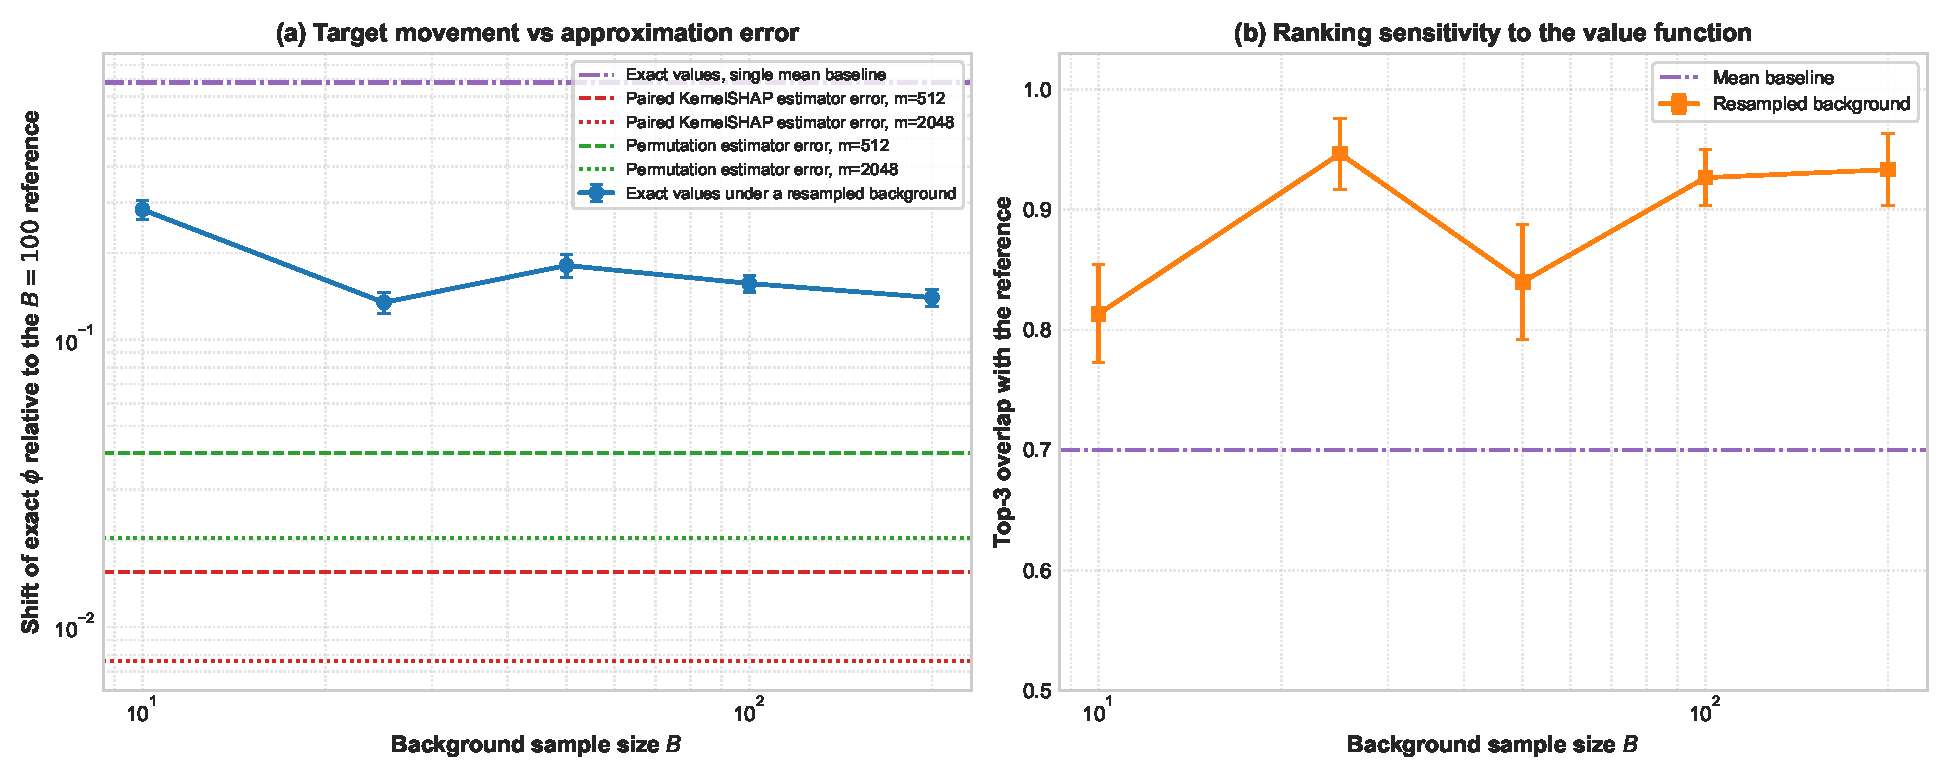
\includegraphics[width=\textwidth]{figures/figure7_value_function_sensitivity.pdf}
\caption{Sensitivity of the exact Shapley values to the background sample. (a) Relative shift of the exact values when the background is replaced (blue), against the relative error of two estimators at two budgets (horizontal lines). (b) Overlap of the top three features with the reference.}
\label{fig:valuefn}
\end{figure*}

\begin{table}[t]
\caption{Shift of the exact values when the background of the value function changes, relative to the $B=100$ reference ($d=12$; 10 instances, 5 resampled backgrounds per size).}
\label{tab:valuefn}
\centering
\small
\resizebox{\columnwidth}{!}{%
\begin{tabular}{lcc}
\toprule
Background & Relative shift & Top-3 overlap \\
\midrule
Single mean baseline & $0.783\pm0.081$ & 0.700 \\
$B=10$ & $0.283\pm0.022$ & 0.813 \\
$B=25$ & $0.134\pm0.011$ & 0.947 \\
$B=50$ & $0.181\pm0.016$ & 0.840 \\
$B=100$ (new draw) & $0.157\pm0.010$ & 0.927 \\
$B=200$ & $0.140\pm0.010$ & 0.933 \\
\bottomrule
\end{tabular}}
\end{table}

Approximation error is only one of two reasons why an estimate can differ from ``the'' Shapley value. The other is that the target itself depends on how missing features are filled in. We recomputed the exact values with a different background sample for each instance and compared them with the original, which used 100 particular training rows (Table~\ref{tab:valuefn}, Fig.~\ref{fig:valuefn}). A single mean baseline moves the values by 78\% of their norm, and only 70\% of the top-3 features survive the change. Resampled backgrounds of 25 to 200 rows shift the exact values by 13--18\%, and the shift does not shrink as $B$ grows past 25. That plateau is expected, since the reference is itself a draw of 100 rows and carries its own sampling noise, so we cannot claim that the true population value lies within that distance of the reference. The point is a comparison of scales. The movement of the target caused by merely redrawing the background is of the order of 0.14--0.18, whereas the error of paired KernelSHAP at $m=2048$ is 0.0076 and that of permutation sampling is 0.020. The target moves roughly twenty times more than the best estimator's error at $m=2048$ and about seven times more than the weakest one's. In this setting, spending more evaluations on the estimator while keeping a small background does not seem a good use of compute. The sensitivity of top-3 membership (0.84--0.95) points the same way.

\subsection{Uncertainty and the gap between ranking and values}
\label{sec:unc}
\begin{figure*}[t]
\centering
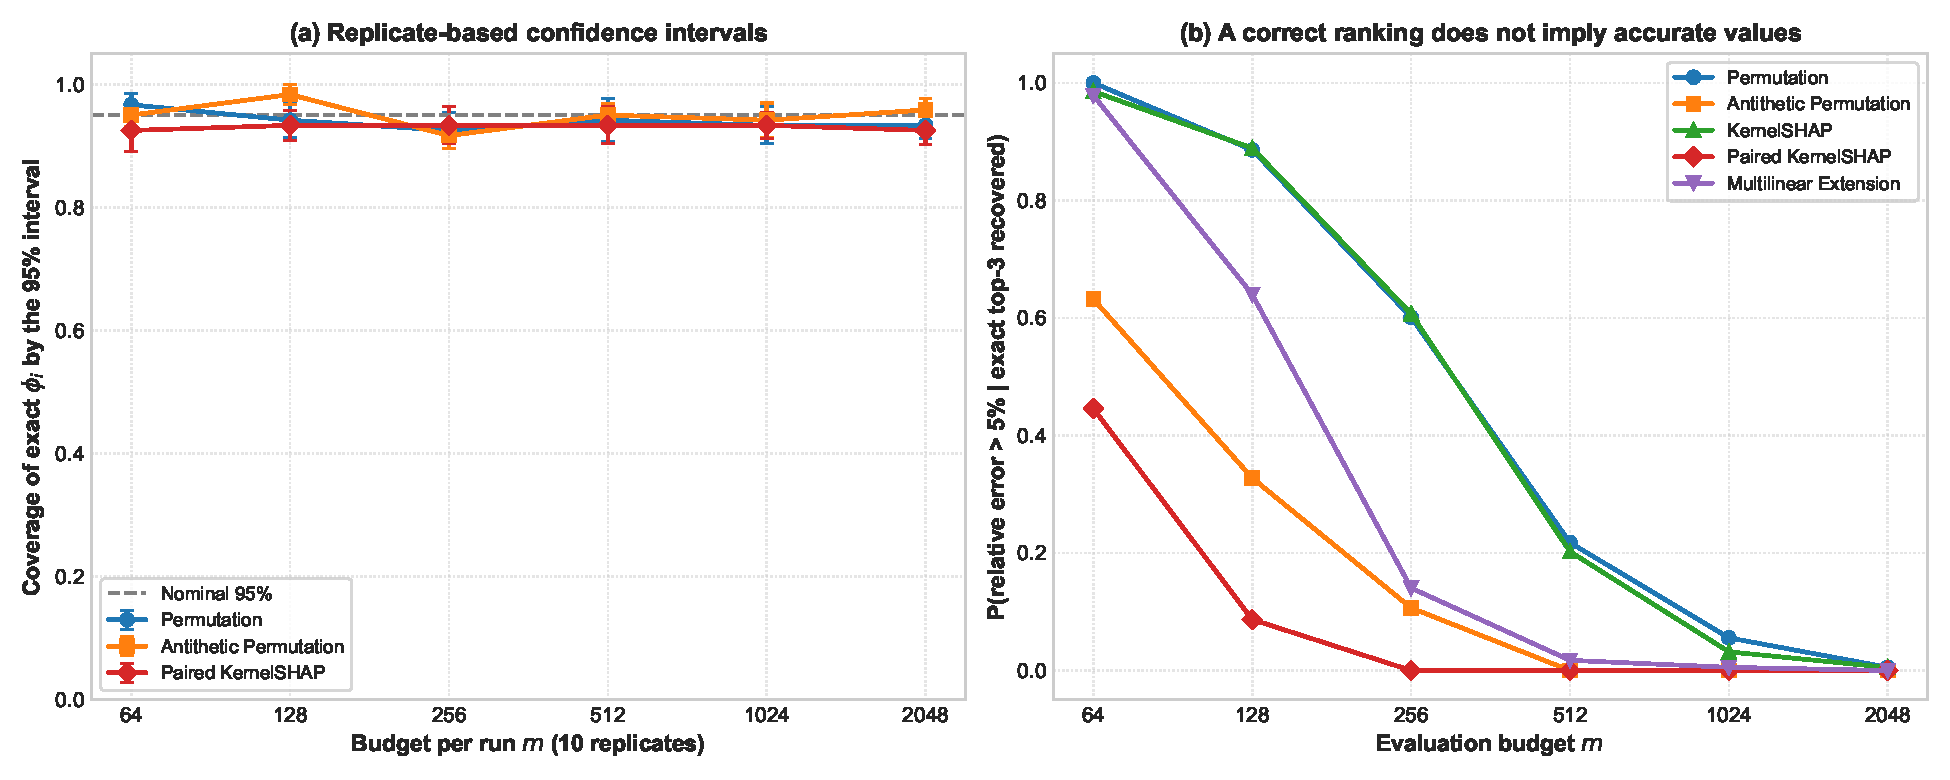
\includegraphics[width=\textwidth]{figures/figure8_uncertainty_and_ranking_gap.pdf}
\caption{(a) Fraction of exact Shapley values that fall inside a 95\% $t$-interval built from 10 independent runs of the estimator. (b) Among runs that recovered the exact top three, the fraction with relative error above 5\%.}
\label{fig:unc}
\end{figure*}

\begin{table}[t]
\caption{Coverage of exact values by 95\% intervals computed from 10 runs ($d=12$; mean over 10 instances $\times$ 12 features; standard error $\approx0.02$--$0.03$ per cell).}
\label{tab:cov}
\centering
\small
\resizebox{\columnwidth}{!}{%
\begin{tabular}{lccccc}
\toprule
Estimator & $m=64$ & $m=256$ & $m=1024$ & $m=2048$ & mean \\
\midrule
Permutation & 0.967 & 0.925 & 0.933 & 0.933 & 0.940 \\
Antithetic perm.\ & 0.950 & 0.917 & 0.942 & 0.958 & 0.958 \\
Paired KernelSHAP & 0.925 & 0.933 & 0.933 & 0.925 & 0.931 \\
\bottomrule
\end{tabular}}
\end{table}

Sampling estimators return random numbers, but attribution plots rarely show an error bar. We checked how well a simple version works. For each instance, we ran an estimator 10 times with independent seeds, formed a 95\% $t$-interval for each feature from the sample mean and standard error, and counted how often the exact value was inside (Table~\ref{tab:cov}, Fig.~\ref{fig:unc}a). Coverage was between 0.92 and 0.98 for the two permutation estimators and between 0.925 and 0.933 for paired KernelSHAP, so close to nominal but, for the regression-based estimator, consistently a little under it, which fits its small finite-sample bias. The price is ten times the budget per explanation. We did not try to build an interval from a single run.

The second question is whether a stable ranking implies accurate numbers (Fig.~\ref{fig:unc}b). Among runs that recovered the exact top three features, we counted how many still had a relative error above 5\%. For permutation sampling the fraction is 0.60 at $m=256$ and 0.22 at $m=512$; for KernelSHAP it is 0.61 and 0.20. At $m=1024$ it is still 0.056 and 0.032, respectively. For antithetic permutation sampling it falls to zero at $m=512$, and for paired KernelSHAP it is zero from $m=256$, although at $m=64$ it is 0.45. A top-3 chart that matches the exact ranking, produced by an unpaired estimator at a few hundred evaluations, is therefore not evidence that the numbers are within five percent. With paired sampling the two coincide earlier.

\section{Discussion and Limitations}
In this benchmark, pairing samples helped every estimator it was applied to, and it takes only a few lines of code. Paired KernelSHAP had the lowest error at every budget and both dimensions we measured, and its top-3 agreement was at or near the best. At $m=2048$ it removed about 63\% of the error of plain KernelSHAP, which corresponds to a sixfold saving in evaluations relative to permutation sampling. If the model is a tree ensemble, TreeSHAP \cite{lundberg2020trees} avoids sampling error altogether; our setting uses a tree ensemble only because its exact values are convenient to tabulate.

Several limitations apply. We used one dataset, one model class and one value function. A depth-4 boosted model has limited high-order interactions, so ratios between estimators may differ for deep networks. Twelve and sixteen features are small enough for brute force but far from the settings in which the approximations are needed, and the $d=16$ study uses five instances. Tabulating the value function made lookups free; for a large model each lookup costs a forward pass on every background point, and the plateau we saw for the background size would then cost real compute. The study explains one scalar output with an interventional value function that evaluates the model on combinations of feature values that may not occur together. With features correlated at $r\approx0.98$, many of those combinations are off the data manifold, and the credit split between near-duplicate features reflects the model's habits more than the data. Conditional value functions \cite{aas2021,frye2021} would address that at an extra cost that we did not measure. More generally, the axioms were designed for dividing a payoff, and several quantities share the name Shapley value for explanation \cite{sundararajan2020many,kumar2020}. Explanations can also be manipulated by exploiting how they are sampled \cite{slack2020}, and Shapley-based feature scores can mislead about which features matter for a decision \cite{huang2024}. The newest estimators, leverage-score and regression-adjusted sampling \cite{musco2025,witter2025} and the improved KernelSHAP weighting \cite{olsen2024}, were not part of our comparison and could be tested with the same protocol. Finally, our convergence-check and interval results are small-sample statements (10 instances; one seed pair, or 10 replicates), and Table~\ref{tab:cov} shows coverage near but not exactly at the nominal level.

\section{Conclusion}
Measured against exact values, paired KernelSHAP was the best of five model-agnostic estimators at every budget and at both problem sizes, reaching 0.76\% relative error with half the evaluations that exact computation needs at twelve features and doing so with about one sixth of the evaluations permutation sampling requires for the same accuracy. All sampling estimators converge at the Monte Carlo rate, so the only real lever is the constant. The multilinear estimator behaves differently from what its efficiency gap first suggests: with four grid points it has a small bias floor, and with finer grids the gap is largely noise. The checks on the setting gave the more important results. The features were strongly collinear, redrawing the background moved the exact values far more than any estimator's error, and rankings from unpaired estimators looked right well before the values did. We suggest reporting an estimator's budget, its seed-to-seed spread and the value function it targets, in addition to its error against exact values.

\section*{Acknowledgment}
The authors thank the Department of Artificial Intelligence at SVNIT, Surat, for guidance on the scope of this study.

\bibliographystyle{IEEEtran}
\bibliography{references}

\end{document}
